% Number 630
% BFPM UFPM Tension FBD
% Half Atwood - conceptual FBD question - frictionlessness maybe too tricky
% JG

% Watermark
\AddToShipoutPicture*{\BackgroundPic}

\addtocounter {ProbNum} {1}

\begin{floatingfigure}[r]{.2\textwidth}
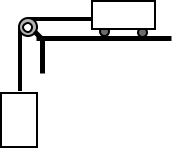
\includegraphics[scale=.6]{/Users/jgates/desktop/latex/pics/halfatwood2}
\end{floatingfigure}
 
{\bf \Large{\arabic{ProbNum}}} A 2 kg cart sits on a table. It is connected by a massless string to a hanging 1 kg box. 
 
\bigskip
Draw force diagrams for the cart and the box after the system is released from rest.  Make the force vector lengths proportional to the sizes of the forces, as best you can.\paragraph{}
\noindent
\vfill
A 5 kg box is now placed on top of the 2 kg cart.  The surfaces of both are frictionless.

Draw force diagrams for all three objects after the system is released from rest.

\vfill

\emph{Without doing any calculations}, do the following quantities increase, decrease, or stay the same as in the original situation?


The weight of the 2 kg cart: \framebox[.5cm][t]{\vphantom{.5cm} } 

\bigskip
The tension in the string: \framebox[.5cm][t]{\vphantom{.5cm} }
 
 \bigskip
The normal force between the table and 2kg cart: \framebox[.5cm][t]{\vphantom{.5cm} } 

\bigskip

%\hfill 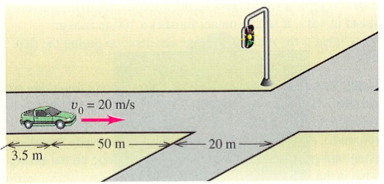
\includegraphics[scale=.85]{/Users/jgates/desktop/latex/pics/redlight.png}
\newpage